\documentclass[10pt,letterpaper]{article}
\usepackage[a4paper, total={6.5in, 8in}]{geometry}
\usepackage{graphicx}
\usepackage{multicol}
\usepackage{verbatim}
\usepackage{tikz}
\usepackage{circuitikz}
\usepackage{float}
\usepackage{dirtytalk}
\usepackage{subcaption}
\usepackage{color}   %May be necessary if you want to color links
\usepackage{hyperref}
\hypersetup{
	colorlinks=true, %set true if you want colored links
	linktoc=all,     %set to all if you want both sections and subsections linked
	linkcolor=blue,  %choose some color if you want links to stand out
	urlcolor=blue
}
\title{Computer Architecture Processor\\
	\large ECE09243: Computer Architecture\\
Dr. Chakraborty}

\author{Stephanie DeMattheis, Aysha Sohail, Jimmy Sunbury, Alexandria Ordoveza\\
Group: RISC-Y Buisness}
\begin{document}
\centering
\maketitle
\newpage
\raggedright
\section{Overview of Features}
\begin{itemize}
	\item A lightning fast 32x32 register file
	\item Extreme performance utilizing the RISC-V32I architecture
	\item No non-volatile memory
	\item Reduced power consumption
	\item Support for Loading, Storing, Branches, and most basic arithmetic operations
	\item 32 bit Instruction Words
	\item 23 Supported Instructions from the RISC-V32I Architecture
\end{itemize}
\newpage
\tableofcontents
\newpage
\section{List of Figures}
\listoffigures
\newpage
\section{List of Tables}
\listoftables
\newpage
\section{Register File Design}
\subsection{Description of design:}
The 32 bit long by 32 bit wide RegFile has the ability to asynchronously read and synchronusly write to the RegFile. The register file has the inputs rd, which is the destination register; rs1 and  rs2, which are the registers to read from; clk, in order to make this device partially synchronous; reset, to clear the contents of each register; enable, which allows the register file to be read from and written to; and rw, which dictates whether the registers are being read from (0) or written to (1). The values of the register will only be changed on the falling edge of every clock cycle if the enable bit is turned on. If the reset bit is turned on, the code will iterate through every register in the RegFile and set the contents of to zero. The input rw controls whether a register is being written to or the contents of the register are being read. When the rw input equals zero, that means the contents of the register are being read. This is done by assigning the outputs, out1 and out2 the contents of the registers that are being read from. When rw equals one, that means a register is being written to, with the contents of register rd being assigned the value of din. 

In order to assign values to each register, the data input is given, along with an address of where the data should be stored. The data is then sent through a multiplexer, with the address as the select bits, which determine where it will be written to. The inverse of this is done when reading from the register file, addresses are given as the select bits of two multiplexers, and the requested data is output.
\begin{figure}[H]
	\centering
	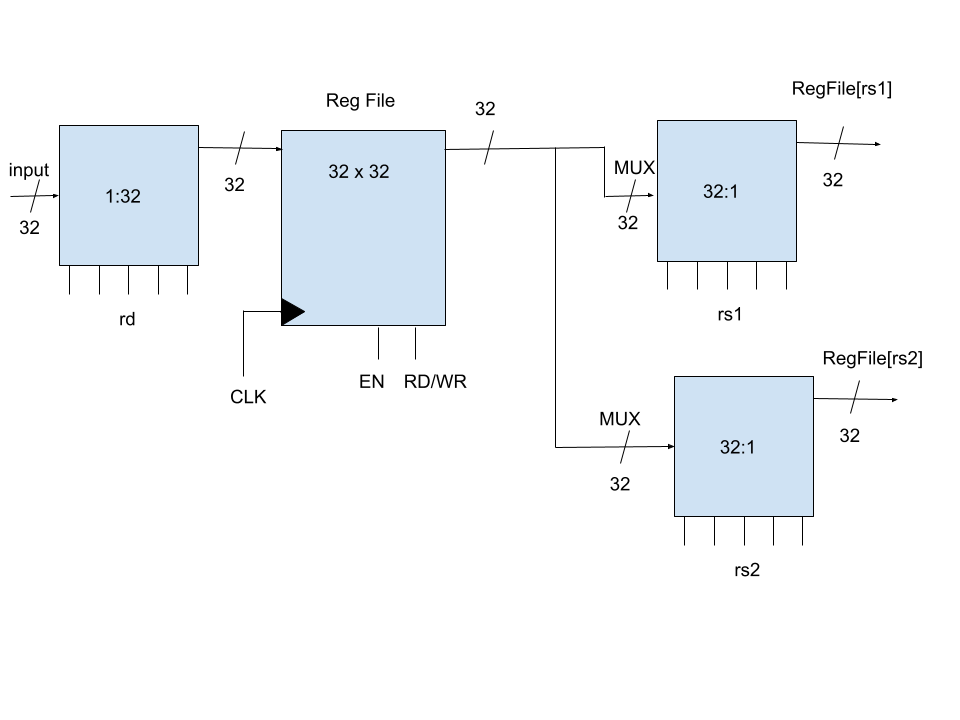
\includegraphics[width=0.7\linewidth]{Figures/RegFileDesign}
	\caption{Block Diagram of Register File Design}
	\label{fig:regfiledesign}
\end{figure}

\subsection{Description and Result of Testbench:}

The testbench in figure \ref*{fig:regfiletb} evaluates and tests the RegFile from figure \ref*{fig:regfiledesign}. The testbench begins by declaring all of the inputs and outputs from the RegFile. The enable, rw, and reset inputs are initialized to one, while the clk is set to zero. A delay occurs and then the reset is set to zero. This means that the rest of the code can execute since reset is not enabled. The din and rd inputs are then set to thirty seven and seventeen respectively. After another delay, the rw input is set to zero, while the rs1 and rs2 inputs are set to seventeen and five. A for loop is then implemented to iterate through all of the registers so that they can be written to with a randomized value  and then read. The loop starts at zero and increments by two, so that the register x and x+1 are written to in one repetition of the loop. At the end of the code, the clk is flipped on and off, so that the rest of the code can execute on the posedge of the clk. 

The output provided by the testbench shows the Register File works as expected. The waveform shows the reset sets the value of the registers to 0, and all of the registers are being correctly written to and read from, as can be seen by the input from a register matching the output after a short delay.
\begin{figure}[H]
	\centering
	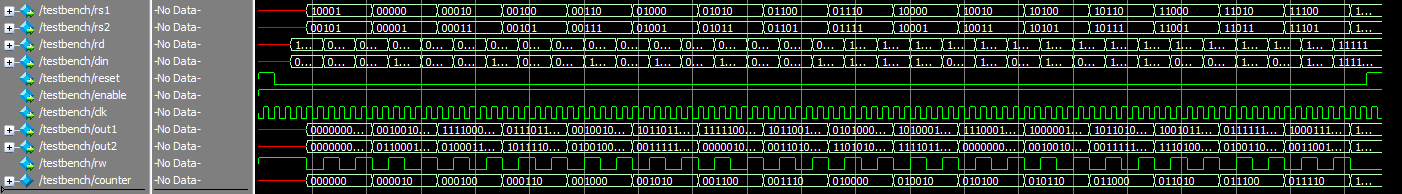
\includegraphics[width=\linewidth]{Figures/RegFileTB}
	\caption{ModelSim Output of RegFile Testbench \href{https://drive.google.com/file/d/16UZ02iNjlCKq06zk10P5jfhbaC_pfCuJ/view?usp=sharing}{$($Link$)$}}
	\label{fig:regfiletb}
\end{figure}
\newpage
\section{Arithmetic and Logic Unit Design}
\subsection{Description of Design}
The ALU has the ability to add, subtract, xor, or, and, and shifting, both arithmetically and logically. The ALU also has status signals such as carry-out, negative, zero, parity (odd), and overflow that get raised when these conditions are met respectively. This design has inputs in1 and in2, which are the first operand and second operand respectively. The last input is op, which is generated by the control unit and decides which operation is to be performed on the operands. Parity is determined by the total number of 1’s in the input. The ALU performs its operations asynchronously, and recalculates the output when either the inputs or operation changes. Each operation has its own case statement, resulting in multiple case statements. In order to decide on the operation, the opcode value is given. 

\begin{figure}[H]
	\centering
	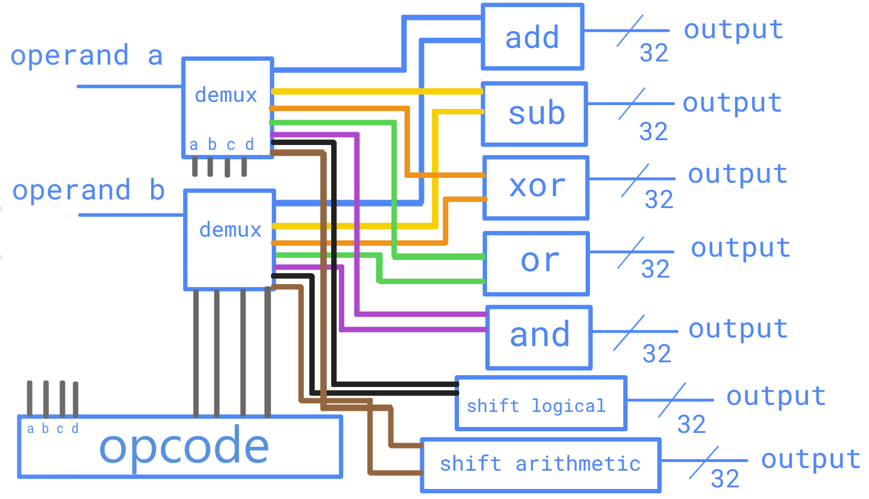
\includegraphics[width=0.7\linewidth]{Figures/ALUDesign1}
	\caption{Diagram of ALU Internals}
	\label{fig:aludesign1}
\end{figure}
\begin{figure}[H]
	\centering
	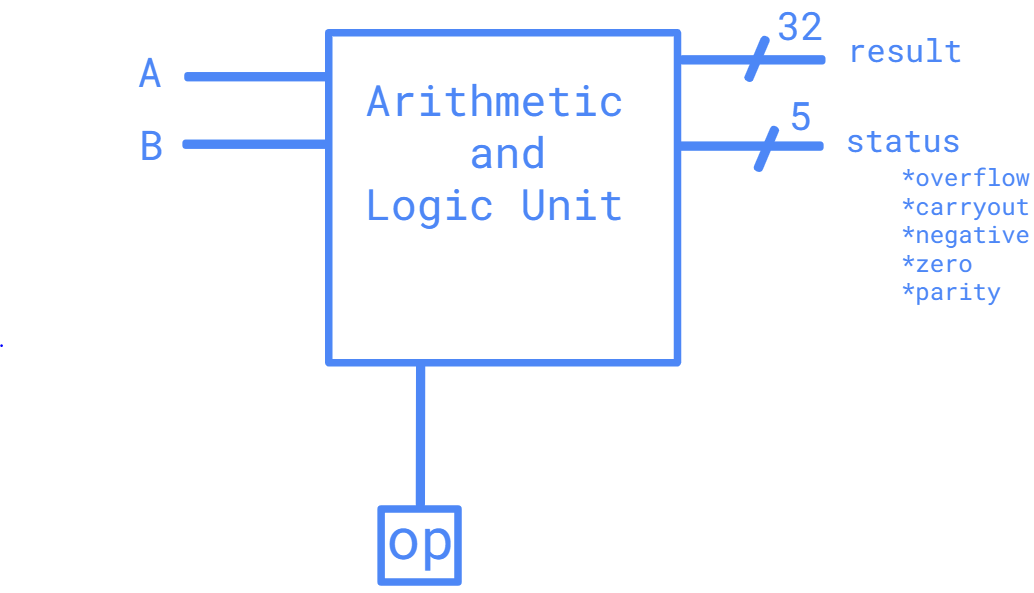
\includegraphics[width=0.7\linewidth]{Figures/ALUDesign2}
	\caption{Block Diagram of ALU}
	\label{fig:aludesign2}
\end{figure}
\begin{table}[H]
	\centering
	\begin{tabular}{|l|l|}
		\hline
		\multicolumn{1}{|c|}{ALU Opcode} & \multicolumn{1}{c|}{Operation} \\ \hline
		0001                             & AND                            \\ \hline
		0010                             & OR                             \\ \hline
		0011                             & XOR                            \\ \hline
		0100                             & ADD                            \\ \hline
		0101                             & SUB                            \\ \hline
		0110                             & SRL                            \\ \hline
		0111                             & SLL                            \\ \hline
		1000                             & SRA                            \\ \hline
		1001                             & SLA                            \\ \hline
		1010                             & ADDU                           \\ \hline
	\end{tabular}
	\caption{ALU Operation Codes}
	\label{tab:opcodes}
\end{table}

\subsection{Description and Result of Testbench:}
The testbench evaluates and tests the functionality of the ALU. The testbench begins by initializing the clk to 0. A short delay occurs and the first input and second input are set to 0101 and 0110 respectively. The opcode is set to 0001 which tests the AND operation. After another delay, the values and operation are changed again, to test OR, then XOR, and finally ADD, with values that would trigger an overflow. The values are then changed once more and all of the operations are tested. Since this is an asynchronous device, the output changes immediately without delay once the inputs are changed.
\begin{figure}[H]
	\centering
	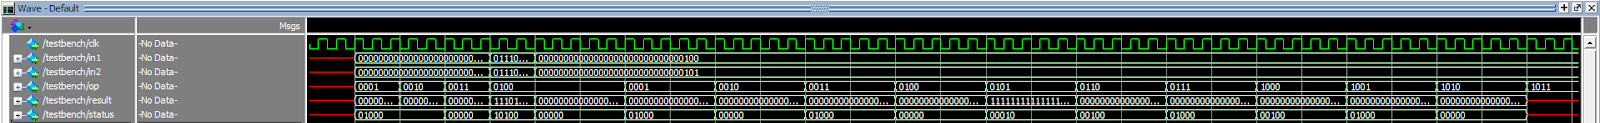
\includegraphics[width=\linewidth]{Figures/ALUTB}
	\caption{ModelSim Output of ALU Testbench \href{https://drive.google.com/file/d/1bQqGJ2kdPRX3t6CaRQ6nDrtCmVe9OP3k/view?usp=sharing}{$($Link$)$}}
	\label{fig:alutb}
\end{figure}
\newpage
\section{Memory Organization}
\subsection{Random Access Memory Design}
\subsubsection{Description of Design:}
RAM, also called Random Access Memory, is the Data Memory of the datapath. The size of our RAM is 32 bits x 2048. Our code is capable of asynchronously reading from and writing to the RAM. In our design, we created eight different chips, each representing a different instantiation of a RAM block. The RAM takes in an input which is the memory address that comes from the Arithmetic and Logic Unit. It also has enable, which allows RAM to be read from and written into. The last input for the RAM is the input value, which comes from the second source register in the RegFile. If read is enabled, the memory address is used as the output of the RAM, and this represents the address we are reading from. If write is enabled, the content of the register is used as the output, and stored into the memory address. 
\begin{figure}[H]
	\centering
	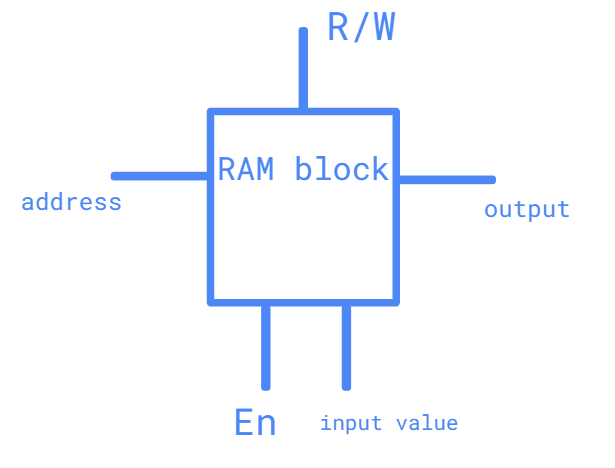
\includegraphics[width=0.7\linewidth]{Figures/RAMDesign}
	\caption{Block Diagram for RAM Block}
	\label{fig:ramdesign}
\end{figure}
\begin{figure}[H]
	\centering
	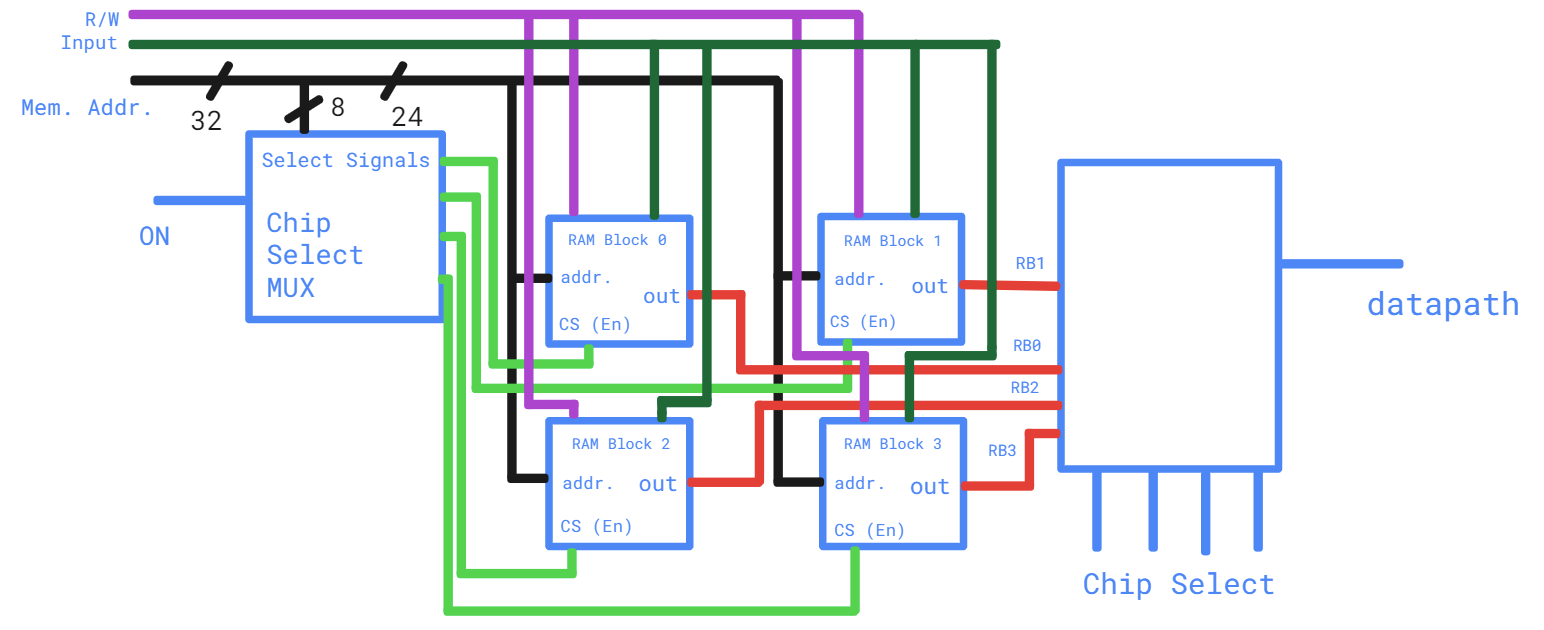
\includegraphics[width=0.7\linewidth]{Figures/RAMDesignComplete}
	\caption{Block Diagram for Complete RAM Unit}
	\label{fig:ramdesigncomplete}
\end{figure}

\subsubsection{Description and Result of Testbench:}
The testbench works by sequentially assigning values to each register in the RAM, and then reading back the written value 3 clock cycles later. In order for the RAM to work, the value written and the value read should be the same. The waveform shown below matched what would be expected, which proved it works.
\begin{figure}[H]
	\centering
	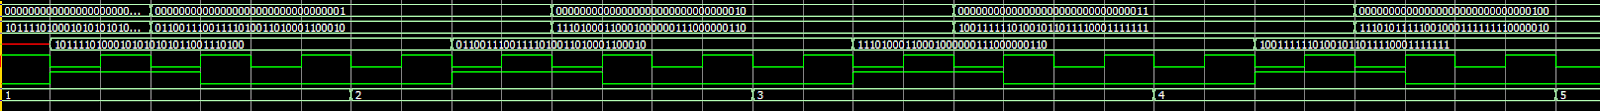
\includegraphics[width=\linewidth]{Figures/RAMTB}
	\caption{ModelSim Output of RAM Testbench \href{https://drive.google.com/file/d/15GmUSFXMRlqQpSEvOUH-_ZZlNqyp-V3_/view?usp=sharing}{$($Link$)$}}
	\label{fig:ramtb}
\end{figure}

\newpage
\subsection{Read Only Memory Design}
\subsubsection{Description of Design:}
ROM, or Read Only Memory, is the Instruction Memory. It can retrieve instructions and send it to the rest of the datapath. It consists of a 8 bit by 128 group of registers. It is byte-addressable and asynchronously reads the values from the ROM and sends it to a 32 bit output. The output is then sent to the regfile, the immediate sign extension mux, and the control unit.
\begin{figure}[H]
	\centering
	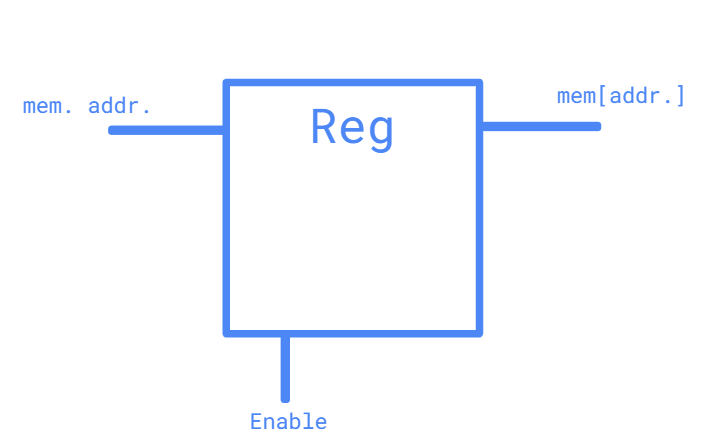
\includegraphics[width=0.7\linewidth]{Figures/ROMDesign}
	\caption{ROM Block Diagram}
	\label{fig:romdesign}
\end{figure}

\subsubsection{Description and Result of Testbench:}
The testbench evaluates the functionality of ROM. The testbench goes through each register and reads the binary values of each group of registers. The values in memory at each address are read, and the output is the 32 bit instruction. This can be seen from the testbench with the top row of numbers indicating the memory address and the second row of numbers indicating the contents of the ROM at that particular 7 bit address. The testbench output was as expected, indicating the ROM functions properly.
\begin{figure}[H]
	\centering
	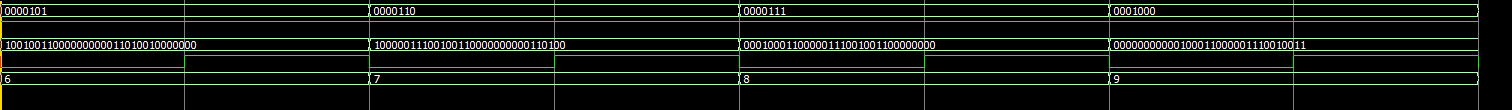
\includegraphics[width=\linewidth]{Figures/ROMTB}
	\caption{ModelSim Output of ROM Testbench \href{https://drive.google.com/file/d/1MDbTakSnFjR1TyeJRE6Qmvgbn0nLsLCv/view?usp=sharing}{$($Link$)$}}
	\label{fig:romtb}
\end{figure}
\newpage
\section{Control Unit Design}
\subsection{Description of Design:}
The control unit consists of different control signals which include: PC Select, RegWEn, ImmSel, BrUn, BEQ, BLT, BSel, ASel, ALUOP, WBSel, and MemRW. It works asynchronously and each signal changes based on the value of the instruction word provided. Each signal has a special purpose. PC Select is 1 if a branch instruction is taken; it is 0 if the branch is not taken. RegWEn is 0 if writing to RegFile is disabled and reading from RegFile is enabled; it is 1 when writing to RegFile is enabled and reading from RegFile is disabled. ImmSel is 0 immediate value is 32-bits long; it is 1 if the immediate value is extended to 32-bits. BrUn is 1 if branch instruction is unsigned; it is 0 if branch is signed. BEQ is 1 if the contents of rs1 and rs2 are equal; it is 0 if they are not equal.  BLT is 1 if the content of rs1 is less than the content of rs2; it is 0 if it is not. BSel is 1 if sign-extended immediate value is selected; it is 0 if rs2 is selected. ASel is 0 if content of rs1 is chosen; it is 1 if the value of the program counter is chosen. ALUOP signal depends on which operation is carried in the instruction word. WBSel is 0 if output of data memory is being written into RegFile; it is 1 if the output came directly from the ALU and is being written into RegFile. MemRW is 1 if it is a store word instruction; it is 0 if it is a load word. In the design, there are five different case statements representing the instruction types which include: R-Type, I-Type, Load Word, Store Word, and Branch instruction. The control signal values depend on the different types of instructions. 
\begin{figure}[H]
	\centering
	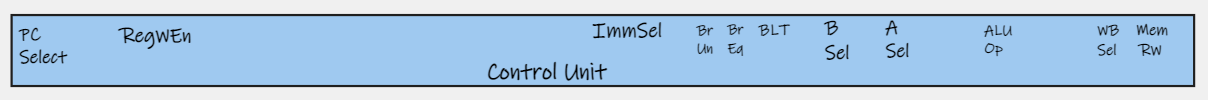
\includegraphics[width=0.7\linewidth]{Figures/ControlUnit}
	\caption{Block Diagram of Control Unit}
	\label{fig:controlunit}
\end{figure}
\begin{table}[H]
	\centering
	\renewcommand{\arraystretch}{2}
	\begin{tabular}{|cc|c|}	
		\hline
		\multicolumn{1}{|c|}{Control Signal Function 1}                                    & Control Signal Function 0                           & Control Signal Name \\ \hline
		\multicolumn{1}{|c|}{\parbox{0.35\textwidth}{\centering Increments the Program Counter by the result of the ALU}}      & \parbox{0.35\textwidth}{\centering Increments the Program Counter by 4}                 & PCSelect            \\ \hline
		\multicolumn{1}{|c|}{\parbox{0.35\textwidth}{\centering Enables the RegFile to be written too}}                        & Disables writing to the RegFile                     & RegWEn              \\ \hline
		\multicolumn{1}{|c|}{\parbox{0.35\textwidth}{\centering Extends the immediate field from 12 bits to 32 bits}}          & \parbox{0.35\textwidth}{\centering \say{Don't Care} output from Immediate Extender}         & ImmSel              \\ \hline
		\multicolumn{1}{|c|}{\parbox{0.35\textwidth}{\centering The top input to the ALU is the value of the Program Counter}} & \parbox{0.35\textwidth}{\centering The top input to the ALU is the value from rs1}      & ASel                \\ \hline
		\multicolumn{1}{|c|}{\parbox{0.35\textwidth}{\centering The bottom input to the ALU is the sign extended immediate}}   & \parbox{0.35\textwidth}{\centering The bottom input to the ALU is the value from rs2}   & BSel                \\ \hline
		\multicolumn{1}{|c|}{\parbox{0.35\textwidth}{\centering The result from the ALU is sent to the RegFile}}               & \parbox{0.35\textwidth}{\centering A value from the Data Memory is sent to the RegFile} & WBSel               \\ \hline
		\multicolumn{1}{|c|}{\parbox{0.35\textwidth}{\centering The Data Memory is able to be written to}}                     & \parbox{0.35\textwidth}{\centering The Data Memory is able to be read from}             & MemRW               \\ \hline
		\multicolumn{1}{|c|}{\parbox{0.35\textwidth}{ \centering The Branch Comparator treats the values of rs1 and rs2 as unsigned}} & \parbox{0.35\textwidth}{ \centering The Branch Comparator treats the values of rs1 and rs2 as signed} & BrUn \\ \hline
		\multicolumn{2}{|c|}{Selects the operation that the ALU performs, specific codes can be seen in table \ref{tab:opcodes}}                                                                       & ALUOP               \\ \hline
	\end{tabular}
	\caption{Control Signals}
	\label{tab:controlsignals}
\end{table}
\subsection{Description and Result of Testbench:}
The testbench evaluates and tests the control unit’s functionality. The testbench decodes the different instruction words and determines the values for the control signals. From the timing diagram below, it clearly works as it shows which bits go to 1 or 0 corresponding to the particular instruction word. The behavior of the timing diagram is what was expected for each of the various instruction words in regards to the different control signals. The blue signals, indicating high impedance are a result of the indeterminate values, such as branch instructions, as the branch comparator is not connected, and therefore, it is unknown whether a branch would be taken. However, the rest of the elements are correct, indicating that the control unit does work properly.

\newpage
\section{CPU and Datapath Design}
\subsection{Description of Design:}
The datapath consists of a Program Counter, RAM, ROM, RegFile, Branch Comparator, Immediate Sign Extension, ALU, and Control Unit. The Program Counter sends the current instruction address to the ROM to get the instruction. The ROM will fetch the instruction and send it to the RegFile to retrieve the register values associated with the instruction. The instruction also is sent to the Immediate sign extension and extends the bits to 12 bits. It also goes to the PC Select bit in the control unit. The output of the RegFile consists of the values stored at RS1 and RS2, which if it is a branch instruction, will go through the branch comparator. The B Sel input is a select bit from the control unit that will decide if the output of the RegFile or the immediate sign extended value will go into the ALU. The ALU will perform the operations based on the control signal from the control unit to give a corresponding output. The ALU output will go into the DMEM module as the address field if the instruction is a load word or store word instruction. For branch instructions, if the branch is taken, the program counter will jump to whatever value was specified in the instruction. Otherwise, it will increment the counter by 4, thereby going to the next instruction.
\begin{figure}[H]
	\centering
	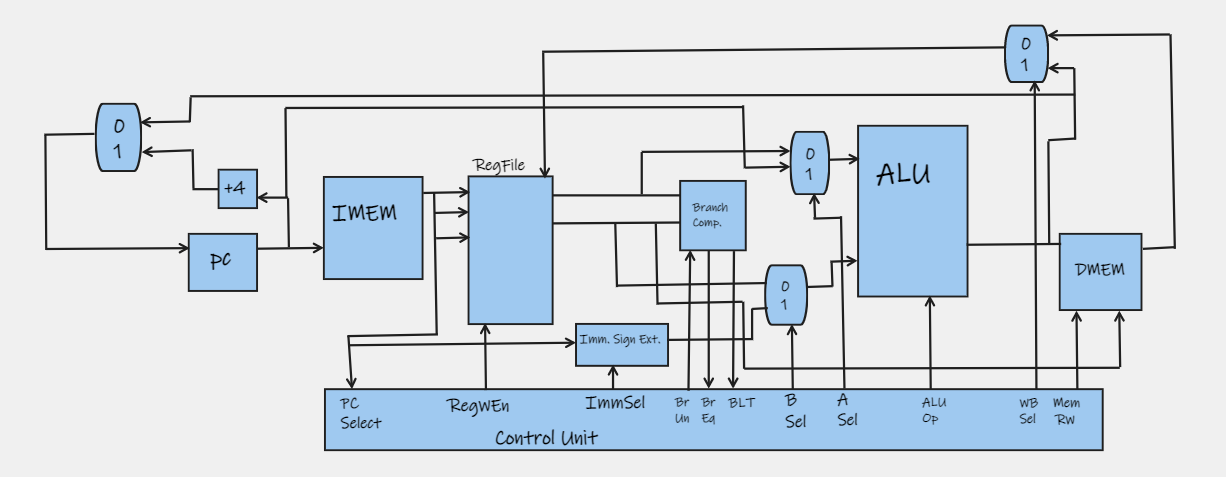
\includegraphics[width=0.7\linewidth]{Figures/DatapathDesign}
	\caption{Block Diagram of Datapath}
	\label{fig:datapathdesign}
\end{figure}

\subsection{Description and Result of Testbench:}
The testbench evaluates how each component of the datapath behaves with one another. The datapath was made by instantiating each component of the datapath as a module and wiring it together. To test the functionality of the datapath, several instructions were fed into the datapath, including ADD, SUB and branch instructions. As can be seen in figure 13, the results were as expected. The commands run were:
\begin{enumerate}
	\item ADDI x9 x9 3
	\item ADDI x3 x3 1
	\item BNE x3 x9 -4
	\item SUB x4 x3 x9 
\end{enumerate}
The final result of this was 0, as expected, because the values of x3 and x9 must be equivalent to avoid taking the branch. The branch was taken twice incrementing x3 to 2, then 3, and then the branch would no longer be taken.
\begin{figure}[H]
	\centering
	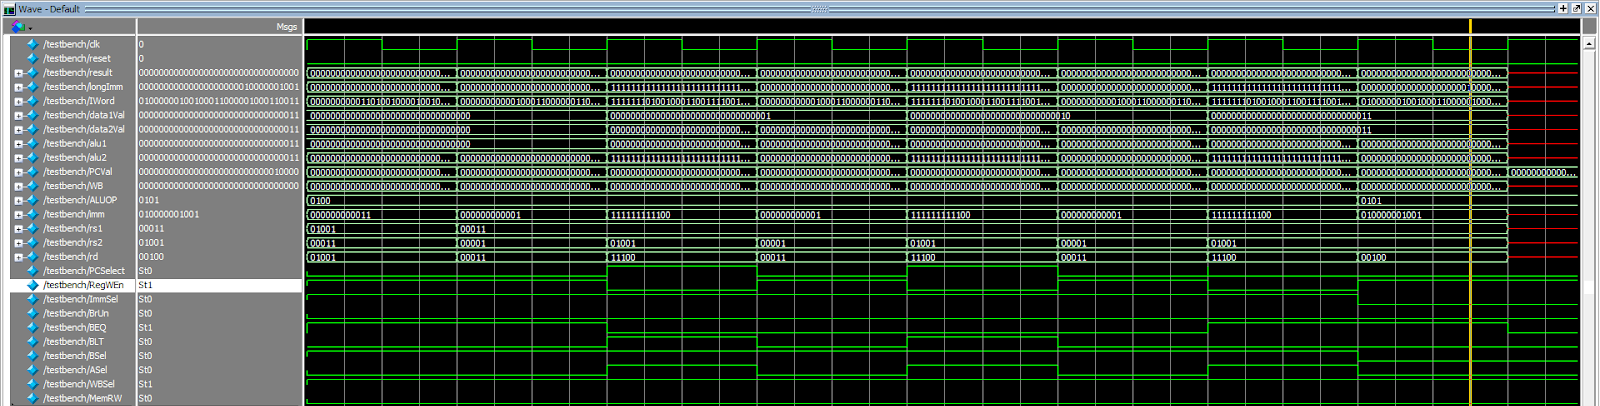
\includegraphics[width=\linewidth]{Figures/DatapathTB}
	\caption{ModelSim Ouput of Datapath TestBench \href{https://drive.google.com/file/d/12lNir8T4gr5fKlothDckKNEPZxD5jp_a/view?usp=sharing}{$($Link$)$}}
	\label{fig:datapathtb}
\end{figure}
\newpage
\section{Instruction Set}
\begin{table}[H]
	\centering
	\begin{tabular}{|crcrcrcrcrcr|c|}
		\hline
		\multicolumn{12}{|c|}{Instruction Word Format} &
		\multicolumn{1}{l|}{} \\ \hline
		\multicolumn{1}{|l}{31} &
		\multicolumn{1}{r|}{25} &
		\multicolumn{1}{l}{24} &
		\multicolumn{1}{r|}{20} &
		\multicolumn{1}{l}{19} &
		\multicolumn{1}{r|}{15} &
		\multicolumn{1}{l}{14} &
		\multicolumn{1}{r|}{12} &
		\multicolumn{1}{l}{11} &
		\multicolumn{1}{r|}{7} &
		\multicolumn{1}{l}{6} &
		0 &
		\multicolumn{1}{l|}{} \\ \hline
		\multicolumn{2}{|c|}{funct7} &
		\multicolumn{2}{c|}{rs2} &
		\multicolumn{2}{c|}{rs1} &
		\multicolumn{2}{c|}{funct3} &
		\multicolumn{2}{c|}{rd} &
		\multicolumn{2}{c|}{opcode} &
		R-Type \\ \hline
		\multicolumn{4}{|c|}{imm{[}11:0{]}} &
		\multicolumn{2}{c|}{rs1} &
		\multicolumn{2}{c|}{funct3} &
		\multicolumn{2}{c|}{rd} &
		\multicolumn{2}{c|}{opcode} &
		I-Type \\ \hline
		\multicolumn{2}{|c|}{imm{[}11:5{]}} &
		\multicolumn{2}{c|}{rs2} &
		\multicolumn{2}{c|}{rs1} &
		\multicolumn{2}{c|}{funct3} &
		\multicolumn{2}{c|}{imm{[}4:0{]}} &
		\multicolumn{2}{c|}{opcode} &
		\begin{tabular}[c]{@{}c@{}}B-Type\\ S-Type\end{tabular} \\ \hline
	\end{tabular}
	\caption{RISC-V32I Instruction Format}
	\label{tab:instrformat}
\end{table}
\begin{table}[H]
	\centering
	\begin{tabular}{|crcrcrcrcrcrc|}
		\hline
		\multicolumn{13}{|c|}{Supported Instruction Set} \\ \hline
		\multicolumn{1}{|l}{31} &
		\multicolumn{1}{r|}{25} &
		\multicolumn{1}{l}{24} &
		\multicolumn{1}{r|}{20} &
		\multicolumn{1}{l}{19} &
		\multicolumn{1}{r|}{15} &
		\multicolumn{1}{l}{14} &
		\multicolumn{1}{r|}{12} &
		\multicolumn{1}{l}{11} &
		\multicolumn{1}{r|}{7} &
		\multicolumn{1}{l}{6} &
		\multicolumn{1}{r|}{0} &
		\multicolumn{1}{l|}{} \\ \hline
		\multicolumn{2}{|c|}{0000000} &
		\multicolumn{2}{c|}{rs2} &
		\multicolumn{2}{c|}{rs1} &
		\multicolumn{2}{c|}{000} &
		\multicolumn{2}{c|}{rd} &
		\multicolumn{2}{c|}{0110011} &
		ADD \\ \hline
		\multicolumn{2}{|c|}{0100000} &
		\multicolumn{2}{c|}{rs2} &
		\multicolumn{2}{c|}{rs1} &
		\multicolumn{2}{c|}{000} &
		\multicolumn{2}{c|}{rd} &
		\multicolumn{2}{c|}{0110011} &
		SUB \\ \hline
		\multicolumn{2}{|c|}{0000000} &
		\multicolumn{2}{c|}{rs2} &
		\multicolumn{2}{c|}{rs1} &
		\multicolumn{2}{c|}{001} &
		\multicolumn{2}{c|}{rd} &
		\multicolumn{2}{c|}{0110011} &
		SLL \\ \hline
		\multicolumn{2}{|c|}{0000000} &
		\multicolumn{2}{c|}{rs2} &
		\multicolumn{2}{c|}{rs1} &
		\multicolumn{2}{c|}{100} &
		\multicolumn{2}{c|}{rd} &
		\multicolumn{2}{c|}{0110011} &
		XOR \\ \hline
		\multicolumn{2}{|c|}{0100000} &
		\multicolumn{2}{c|}{rs2} &
		\multicolumn{2}{c|}{rs1} &
		\multicolumn{2}{c|}{101} &
		\multicolumn{2}{c|}{rd} &
		\multicolumn{2}{c|}{0110011} &
		SRA \\ \hline
		\multicolumn{2}{|c|}{0000000} &
		\multicolumn{2}{c|}{rs2} &
		\multicolumn{2}{c|}{rs1} &
		\multicolumn{2}{c|}{101} &
		\multicolumn{2}{c|}{rd} &
		\multicolumn{2}{c|}{0110011} &
		SRL \\ \hline
		\multicolumn{2}{|c|}{0000000} &
		\multicolumn{2}{c|}{rs2} &
		\multicolumn{2}{c|}{rs1} &
		\multicolumn{2}{c|}{110} &
		\multicolumn{2}{c|}{rd} &
		\multicolumn{2}{c|}{0110011} &
		OR \\ \hline
		\multicolumn{2}{|c|}{0000000} &
		\multicolumn{2}{c|}{rs2} &
		\multicolumn{2}{c|}{rs1} &
		\multicolumn{2}{c|}{111} &
		\multicolumn{2}{c|}{rd} &
		\multicolumn{2}{c|}{0110011} &
		AND \\ \hline
		\multicolumn{4}{|c|}{imm{[}11:0{]}} &
		\multicolumn{2}{c|}{rs1} &
		\multicolumn{2}{c|}{000} &
		\multicolumn{2}{c|}{rd} &
		\multicolumn{2}{c|}{0010011} &
		ADDI \\ \hline
		\multicolumn{4}{|c|}{imm{[}11:0{]}} &
		\multicolumn{2}{c|}{rs1} &
		\multicolumn{2}{c|}{001} &
		\multicolumn{2}{c|}{rd} &
		\multicolumn{2}{c|}{0010011} &
		SLLI \\ \hline
		\multicolumn{4}{|c|}{imm{[}11:0{]}} &
		\multicolumn{2}{c|}{} &
		\multicolumn{2}{c|}{100} &
		\multicolumn{2}{c|}{rd} &
		\multicolumn{2}{c|}{0010011} &
		XORI \\ \hline
		\multicolumn{2}{|c|}{0100000} &
		\multicolumn{2}{c|}{shamt} &
		\multicolumn{2}{c|}{rs1} &
		\multicolumn{2}{c|}{101} &
		\multicolumn{2}{c|}{rd} &
		\multicolumn{2}{c|}{0010011} &
		SRAI \\ \hline
		\multicolumn{2}{|c|}{0000000} &
		\multicolumn{2}{c|}{shamt} &
		\multicolumn{2}{c|}{rs1} &
		\multicolumn{2}{c|}{101} &
		\multicolumn{2}{c|}{rd} &
		\multicolumn{2}{c|}{0010011} &
		SRLI \\ \hline
		\multicolumn{4}{|c|}{imm{[}11:0{]}} &
		\multicolumn{2}{c|}{rs1} &
		\multicolumn{2}{c|}{110} &
		\multicolumn{2}{c|}{rd} &
		\multicolumn{2}{c|}{0010011} &
		ORI \\ \hline
		\multicolumn{4}{|c|}{imm{[}11:0{]}} &
		\multicolumn{2}{c|}{rs1} &
		\multicolumn{2}{c|}{111} &
		\multicolumn{2}{c|}{rd} &
		\multicolumn{2}{c|}{0010011} &
		ANDI \\ \hline
		\multicolumn{4}{|c|}{imm{[}11:0{]}} &
		\multicolumn{2}{c|}{rs1} &
		\multicolumn{2}{c|}{010} &
		\multicolumn{2}{c|}{rd} &
		\multicolumn{2}{c|}{0000011} &
		LW \\ \hline
		\multicolumn{2}{|c|}{imm{[}11:5{]}} &
		\multicolumn{2}{c|}{rs2} &
		\multicolumn{2}{c|}{rs1} &
		\multicolumn{2}{c|}{010} &
		\multicolumn{2}{c|}{imm{[}4:0{]}} &
		\multicolumn{2}{c|}{0100011} &
		SW \\ \hline
		\multicolumn{2}{|c|}{imm{[}11:5{]}} &
		\multicolumn{2}{c|}{rs2} &
		\multicolumn{2}{c|}{rs1} &
		\multicolumn{2}{c|}{000} &
		\multicolumn{2}{c|}{imm{[}4:0{]}} &
		\multicolumn{2}{c|}{0100011} &
		BEQ \\ \hline
		\multicolumn{2}{|c|}{imm{[}11:5{]}} &
		\multicolumn{2}{c|}{rs2} &
		\multicolumn{2}{c|}{rs1} &
		\multicolumn{2}{c|}{001} &
		\multicolumn{2}{c|}{imm{[}4:0{]}} &
		\multicolumn{2}{c|}{0100011} &
		BNE \\ \hline
		\multicolumn{2}{|c|}{imm{[}11:5{]}} &
		\multicolumn{2}{c|}{rs2} &
		\multicolumn{2}{c|}{rs1} &
		\multicolumn{2}{c|}{100} &
		\multicolumn{2}{c|}{imm{[}4:0{]}} &
		\multicolumn{2}{c|}{0100011} &
		BLT \\ \hline
		\multicolumn{2}{|c|}{imm{[}11:5{]}} &
		\multicolumn{2}{c|}{rs2} &
		\multicolumn{2}{c|}{rs1} &
		\multicolumn{2}{c|}{101} &
		\multicolumn{2}{c|}{imm{[}4:0{]}} &
		\multicolumn{2}{c|}{0100011} &
		BGE \\ \hline
		\multicolumn{2}{|c|}{imm{[}11:5{]}} &
		\multicolumn{2}{c|}{rs2} &
		\multicolumn{2}{c|}{rs1} &
		\multicolumn{2}{c|}{110} &
		\multicolumn{2}{c|}{imm{[}4:0{]}} &
		\multicolumn{2}{c|}{0100011} &
		BLTU \\ \hline
		\multicolumn{2}{|c|}{imm{[}11:5{]}} &
		\multicolumn{2}{c|}{rs2} &
		\multicolumn{2}{c|}{rs1} &
		\multicolumn{2}{c|}{111} &
		\multicolumn{2}{c|}{imm{[}4:0{]}} &
		\multicolumn{2}{c|}{0100011} &
		BGEU \\ \hline
	\end{tabular}
	\caption{RISC-V32I Instruction Set Supported by the Processor}
	\label{tab:instrSet}
\end{table}
\newpage
\section{Supported Instruction Details}
\begin{itemize}
	\item R-Type:
		\begin{itemize}
			\item ADD- Adds the values at rs1 and rs2, and stores the result in rd
			\item SUB- Subtracts the values at rs2 from rs1, and stores the result in rd
			\item SLL- Shifts the value at rs1 left by the value in rs2 and stores the result in rd
			\item XOR- XORs the values of rs1 and rs2 and stores the result in rd
			\item SRA- Shifts the value in rs1 right  by the value of rs2, while maintaining the sign, and stores the result in rd
			\item SRL- Shifts the value in rs1 right by the value of rs2 and stores the result in rd
			\item OR- ORs the values in rs1 with those in rs2 and stores the result in rd
			\item AND- ANDs the values in rs1 with rs2 and stores the result in rd
		\end{itemize}



	\item I-Type
	\begin{itemize}
		\item ADDI- Adds the value in the immediate field to the value in rs1 and stores the result in rd
		\item SLLI- Shifts the value stored in rs1 left by the value in the immediate field and stores the result in rd
		\item XORI- XORs the value in rs1 with the value in the immediate field and stores the result in rd
		\item SRAI- Shifts the value in rs1 right by the value in the immediate field, while preserving the sign, and storing the result in rd
		\item SRLI- Shifts the value in rs1 right by the value in the immediate field and storing the result in rd
		\item ORI- ORs the value in rs1 with the value in the immediate field, and stores the result in rd
		\item ANDI- ANDs the value in rs1 with the value in the immediate field and stores the result in rd
	\end{itemize}
	\item Load Instructions
	\begin{itemize}
		\item Load Word- Loads the value in RAM at the address of the value of the immediate field plus the value of rs1 into rd
	\end{itemize}
	\item S-Type Instructions
	\begin{itemize}
		\item Store Word- Stores the value in rs1 into RAM at the address of rs2 plus the value of the immediate field
	\end{itemize}
	\item B-Type Instructions
	\begin{itemize}
		\item BEQ- Compares the value in rs1 and rs2, and if they are equal modifies the program counter by the value in the immediate field
		\item BNE-  Compares the value in rs1 and rs2, and if they are not equal modifies the program counter by the value in the immediate field
		\item BLT- Compares the value in rs1 and rs2, and if rs1 is less than rs2 modifies the program counter by the value in the immediate field
		\item BGE- Compares the value in rs1 and rs2, and if rs1 is greater than or equal to rs2 modifies the program counter by the value in the immediate field
		\item BLTU- Compares the value in rs1 and rs2, ignoring the sign bit, and if rs1 is less than rs2 modifies the program counter by the value in the immediate field
		\item BGEU- Compares the value in rs1 and rs2, ignoring the sign bit, and if rs1 is greater than or equal to rs2 modifies the program counter by the value in the immediate field
	\end{itemize}
\end{itemize}
\newpage
\section{Example Program}
\begin{enumerate}
	\item ADDI x9 x9 33
	\item ADDI x4 x4 1
	\item SRLI x9 x9 1
	\item BLT x4 x9 -8
	\item XORI x7 x4 13 	
\end{enumerate}
This program begins by assigning a value of 33 to x9, then 1 to x4. It then shifts the value stored in x9 left 1, and compares the values stored in x4 and x9, and if x4 is less than x9 the branch will be taken, shifting the value of x9 right by 1 again. Once the value in x4 is greater than or equal to than in x9, x4 is XORed with 13 and the result is stored in x7.
The expected values for the registers are as follows:
\begin{table}[H]
	\centering
	\begin{tabular}{|c|c|c|c|c|c|c|c|c|c|c|c|c|c|c|c|}
		\hline
		\multicolumn{1}{|l|}{} & PC Value 0     & 4  & 8  & 12 & 16 & 8  & 12 & 16 & 8  & 12 & 16 & 8  & 12 & 16 & 20 \\ \hline
		Register               & Initialization & I1 & I2 & I3 & I4 & I2 & I3 & I4 & I2 & I3 & I4 & I2 & I3 & I4 & I5 \\ \hline
		x4                     & 0              & 0  & 1  & 1  & 1  & 2  & 2  & 2  & 3  & 3  & 3  & 4  & 4  & 4  & 4  \\ \hline
		x7                     & 0              & 0  & 0  & 0  & 0  & 0  & 0  & 0  & 0  & 0  & 0  & 0  & 0  & 0  & 9  \\ \hline
		x9                     & 0              & 33 & 33 & 16 & 16 & 16 & 8  & 8  & 8  & 4  & 4  & 4  & 2  & 2  & 2  \\ \hline
	\end{tabular}
	\caption{Sample Program Expected Results}
\end{table}
\begin{figure}[H]
	\centering
	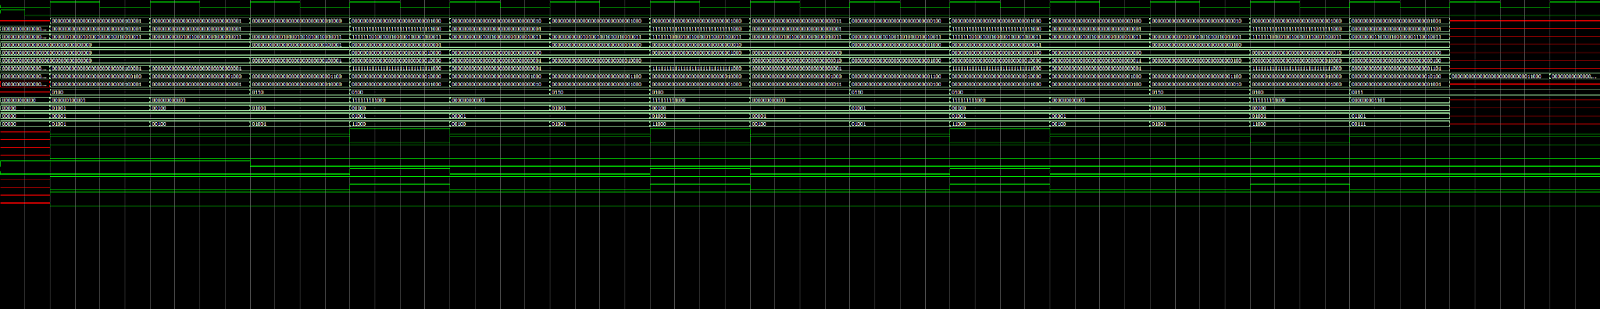
\includegraphics[width=\linewidth]{Figures/SampleProgram}
	\caption{Sample Program Output \href{https://drive.google.com/file/d/1mjlTnk4JS1E0iR5rboaUu_RLDmP1-2R1/view?usp=sharing}{$($Link$)$}}
	\label{fig:sampleprogram}
\end{figure}

As the simulation shows, the sample program’s output matched exactly with the expected behavior, verifying that the CPU works, and the elements composing it work.
\newpage
\section{Performance}
The CPU created in this class functions extremely well as a proof of concept and a demonstration of the understanding of the concepts of this course, however compared to modern day CPUs and microcontrollers it falls very short. The most significant drawback of this CPU is the lack of pipelining. As only 1 instruction can be processed at a time, there are many elements that are only in use for a brief time, which do nothing once they’ve fulfilled their purpose. Pipelining would greatly improve the IPC as these previously underutilized modules would be constantly performing their operations. IPC is however only one of the standards on which the performance of the CPU can be measured. While this CPU also does not interact with many tiers of the memory hierarchy, the performance could be further improved by adding a cache in order to fetch commonly used values more quickly than RAM, however slower than the registers built into the RegFile. This is, however, a less straightforward performance improvement as it largely depends on the program that is being executed; a program that makes many calls to memory would likely experience a far greater effect than a program that’s computation only relies on a few values. Another limitation of this CPU is the size of the instruction and data memory, abiding by the RV32I architecture, the RegFile’s size cannot be increased, as the instruction words would be unable to reference addresses greater than 32, but data memory and instruction memory could be greatly increased in size to accommodate larger programs, in both literal size, and complexity. 
\end{document}